%% =====================================================================
%%  Capítulo de L. Forzani, actualizado por la autora (2026-10) e integrado
%%  al apunte: preámbulo, macros y bibliografía viven en main.tex.
%% =====================================================================
\chapter{Análisis discriminante lineal (LDA)}\label{cap:lda}\label{lda-cap}

% =====================================================================
\section{Introducción}\label{lda-sec:intro}

En el capítulo anterior clasificamos con la regla más simple: resumir cada
clase con su media y asignar una observación nueva a la clase cuya media está
más cerca. En los ocho puntos de ese capítulo la regla acierta $6$ de los $8$
puntos, aunque las dos clases se pueden separar perfectamente con una recta
inclinada; y PCA no ayuda, porque la dirección de máxima varianza mezcla las
clases. Las dos cosas fallan por lo mismo: miran las medias, o la nube entera,
pero no la \emph{forma} de cada clase.

La idea de Fisher \cite{Fisher1936}, de 1936, es buscar directamente la
dirección en la que \emph{las medias de las clases proyectadas quedan lo más
separadas posible en relación con lo que se desparrama cada clase
proyectada}. Con esa dirección se clasifica como antes: se proyecta y se usa
la media más cercana. El método se llama \textbf{análisis discriminante
lineal} (LDA, por su nombre en inglés, \emph{linear discriminant analysis}).

Lo que más nos interesa es la matemática que hay detrás. Escrito con
matrices, el problema de Fisher es maximizar un cociente de dos formas
cuadráticas, $\bi{w}\transp A\bi{w}/\bi{w}\transp B\bi{w}$: un \textbf{cociente de Rayleigh
generalizado} (Sección I.10 de \cite{Strang2019}). No usamos teoría
estadística (en estadística, LDA se deduce de un modelo probabilístico para
las clases; acá no nos hace falta). El plan:
\begin{enumerate}[leftmargin=*,itemsep=1pt]
\item con dos clases, el cociente de Fisher, escrito con matrices
(Sección~\ref{lda-sec:fisher});
\item el teorema general: el cociente de Rayleigh generalizado
(Sección~\ref{lda-sec:rayleigh});
\item la dirección de Fisher, como caso particular de ese teorema
(Sección~\ref{lda-sec:direccion}), y cómo se clasifica con ella
(Sección~\ref{lda-sec:clasificar});
\item más de dos clases, que es aplicar el mismo teorema, y una comparación
con PCA (Sección~\ref{lda-sec:multi});
\item otra aplicación del mismo teorema: diagonalizar dos formas cuadráticas
a la vez (Sección~\ref{lda-sec:simultanea}).
\end{enumerate}

% =====================================================================
\section{Dos clases: el cociente de Fisher}\label{lda-sec:fisher}

Usamos la notación del capítulo anterior: $X\in\R^{n\times p}$ tiene las
observaciones $\bi{x}_1\transp,\dots,\bi{x}_n\transp$ en las filas, $y_i\in\{1,\dots,C\}$
es la clase de la observación $i$, la clase $k$ tiene $n_k$ observaciones y
media $\bar{\bi{x}}_k$, y $\bar{\bi{x}}$ es la media de todos los datos. En las
Secciones~\ref{lda-sec:fisher} a~\ref{lda-sec:clasificar} hay dos clases
($C=2$); la Sección~\ref{lda-sec:rayleigh} es la herramienta general.

\paragraph{Proyectar sobre una dirección.} Dado un vector $\bi{w}\ne0$, cada
observación $\bi{x}$ se resume con un número, $\bi{w}\transp \bi{x}$ (si $\|\bi{w}\|=1$, es la
coordenada de la proyección de $\bi{x}$ sobre la recta $\gen(\bi{w})$, como un score de
PCA). La media de los números $\bi{w}\transp \bi{x}_i$ de la clase $k$ es el número de la
media: $\frac1{n_k}\sum_{i:\,y_i=k}\bi{w}\transp \bi{x}_i=\bi{w}\transp\bar{\bi{x}}_k$. Para que las
clases queden separadas en la recta nos interesan dos cosas:
\begin{itemize}[leftmargin=*,itemsep=1pt]
\item que las \textbf{medias proyectadas} queden lejos, es decir, que
$(\bi{w}\transp\bar{\bi{x}}_1-\bi{w}\transp\bar{\bi{x}}_2)^2$ sea grande;
\item que cada \textbf{clase proyectada} se desparrame poco alrededor de su
media proyectada, es decir, que
\[
\sum_{k=1}^{2}\ \sum_{i:\ y_i=k}\bigl(\bi{w}\transp \bi{x}_i-\bi{w}\transp\bar{\bi{x}}_k\bigr)^2
\]
sea chica.
\end{itemize}

\paragraph{Las dos cantidades, con matrices.} Las dos son \emph{formas
cuadráticas} en $\bi{w}$, es decir, de la forma $\bi{w}\transp M\bi{w}$ con $M$ simétrica.

\emph{Las medias proyectadas.} Sea $\bi{a}=\bar{\bi{x}}_1-\bar{\bi{x}}_2\in\R^p$. Entonces
$\bi{w}\transp\bar{\bi{x}}_1-\bi{w}\transp\bar{\bi{x}}_2=\bi{w}\transp \bi{a}$ es un número (una matriz de
$1\times p$ por una de $p\times1$), igual a su transpuesto $\bi{a}\transp \bi{w}$, y
\[
(\bi{w}\transp\bar{\bi{x}}_1-\bi{w}\transp\bar{\bi{x}}_2)^2=(\bi{w}\transp \bi{a})(\bi{a}\transp \bi{w})=\bi{w}\transp\,(\bi{a}\bi{a}\transp)\,\bi{w} .
\]
La matriz $\bi{a}\bi{a}\transp\in\R^{p\times p}$ es simétrica, de rango uno y
semidefinida positiva.

\emph{Las clases proyectadas.} Sea $\tilde X\in\R^{n\times p}$ la matriz cuya fila
$i$ es $(\bi{x}_i-\bar{\bi{x}}_{y_i})\transp$: cada observación menos la media de su
clase. Entonces
\[
\tilde X\bi{w}=\begin{pmatrix}(\bi{x}_1-\bar{\bi{x}}_{y_1})\transp\\ \vdots\\ (\bi{x}_n-\bar{\bi{x}}_{y_n})\transp\end{pmatrix}\bi{w}
=\begin{pmatrix}\bi{w}\transp \bi{x}_1-\bi{w}\transp\bar{\bi{x}}_{y_1}\\ \vdots\\ \bi{w}\transp \bi{x}_n-\bi{w}\transp\bar{\bi{x}}_{y_n}\end{pmatrix}\in\R^n
\]
tiene en la entrada $i$ cuánto se aleja la observación $i$ proyectada de la
media proyectada de su clase, y la suma de arriba es la suma de los cuadrados
de esas entradas:
\[
\sum_{k=1}^{2}\ \sum_{i:\ y_i=k}\bigl(\bi{w}\transp \bi{x}_i-\bi{w}\transp\bar{\bi{x}}_k\bigr)^2
=\|\tilde X\bi{w}\|^2=(\tilde X\bi{w})\transp(\tilde X\bi{w})=\bi{w}\transp\,(\tilde X\transp \tilde X)\,\bi{w} .
\]

\begin{definition}[Dispersión dentro de las clases]\label{lda-def:SW}
La \textbf{matriz de dispersión dentro de las clases} es
\[
S=\tilde X\transp \tilde X=\sum_{k}\ \sum_{i:\ y_i=k}(\bi{x}_i-\bar{\bi{x}}_k)(\bi{x}_i-\bar{\bi{x}}_k)\transp\ \in\R^{p\times p}.
\]
Es simétrica y semidefinida positiva, porque $\bi{w}\transp S\bi{w}=\|\tilde X\bi{w}\|^2\ge0$.
\end{definition}

\begin{remark}[¿Cuándo es invertible?]\label{lda-rem:invertible}
Si $S\bi{w}=0$, entonces $\|\tilde X\bi{w}\|^2=\bi{w}\transp S\bi{w}=0$, es decir, $\tilde X\bi{w}=0$; y al
revés, si $\tilde X\bi{w}=0$, entonces $S\bi{w}=\tilde X\transp \tilde X\bi{w}=0$. Así que $S$ es
invertible si y solo si $\tilde X$ tiene rango $p$, y en ese caso es
\emph{definida positiva}: $\bi{w}\transp S\bi{w}>0$ para todo $\bi{w}\ne0$. Como las filas
de $\tilde X$ de cada clase suman cero, $\rango(\tilde X)\le n-C$
(Ejercicio~\ref{lda-ej:SW}): si hay más variables que datos, $S$ no es
invertible. En todo el capítulo suponemos que $S$ es invertible.
\end{remark}

\begin{definition}[Cociente de Fisher]\label{lda-def:fisher}
Si $S$ es invertible, para $\bi{w}\ne0$ el \textbf{cociente de Fisher} es
\[
J(\bi{w})=\frac{(\bi{w}\transp\bar{\bi{x}}_1-\bi{w}\transp\bar{\bi{x}}_2)^2}{\displaystyle\sum_{k=1}^{2}\ \sum_{i:\ y_i=k}\bigl(\bi{w}\transp \bi{x}_i-\bi{w}\transp\bar{\bi{x}}_k\bigr)^2}
=\frac{\bi{w}\transp(\bi{a}\bi{a}\transp)\bi{w}}{\bi{w}\transp S\bi{w}},\qquad \bi{a}=\bar{\bi{x}}_1-\bar{\bi{x}}_2 .
\]
\end{definition}

Queremos el numerador grande (las medias proyectadas lejos) y el denominador
chico (cada clase proyectada compacta): $J(\bi{w})$ mide la separación de las
medias proyectadas \emph{en relación con} la dispersión de las clases
proyectadas. Como numerador y denominador quedan multiplicados por $c^2$ al
cambiar $\bi{w}$ por $c\bi{w}$, $J(c\bi{w})=J(\bi{w})$ para todo $c\ne0$: solo importa la
dirección. Y escrito así, $J$ es un cociente de dos formas cuadráticas, con la
matriz $\bi{a}\bi{a}\transp$ arriba y la matriz $S$ abajo: es el problema de la
próxima sección.

\begin{example}[Los ocho puntos]\label{lda-ejem:ocho}
En los ocho puntos del capítulo anterior, la clase~1 es $(2,3)$, $(1,3)$,
$(-1,-3)$, $(-2,-3)$, con media $\bar{\bi{x}}_1=(0,0)$, y la clase~2 es la clase~1
trasladada en $(3,0)$, con media $\bar{\bi{x}}_2=(3,0)$. Entonces
\[
\bi{a}=\begin{pmatrix}-3\\0\end{pmatrix},\qquad \bi{a}\bi{a}\transp=\begin{pmatrix}9&0\\0&0\end{pmatrix}.
\]
Restando a cada punto la media de su clase quedan, en las dos clases, los
mismos cuatro vectores $(2,3)$, $(1,3)$, $(-1,-3)$, $(-2,-3)$, así que
\[
\tilde X=\begin{pmatrix}2&1&-1&-2&2&1&-1&-2\\3&3&-3&-3&3&3&-3&-3\end{pmatrix}\transp,\qquad
S=\tilde X\transp \tilde X=\begin{pmatrix}20&36\\36&72\end{pmatrix}.
\]
Comparemos algunas direcciones:
\begin{itemize}[leftmargin=*,itemsep=1pt]
\item $\bi{e}_1=(1,0)$, la dirección de la recta que une las medias, que es la que
usa la regla de la media más cercana: $J(\bi{e}_1)=9/20=0{,}45$;
\item $\bi{v}_1\approx(0{,}535;\,0{,}845)$, la primera dirección principal:
$J(\bi{v}_1)\approx2{,}58/89{,}7\approx0{,}029$;
\item $\bi{v}_2\approx(0{,}845;\,-0{,}535)$, la segunda dirección principal, que en
el capítulo anterior separaba las clases: $J(\bi{v}_2)\approx6{,}42/2{,}34\approx2{,}74$.
\end{itemize}
¿Hay una dirección mejor que $\bi{v}_2$? Sí: en la Sección~\ref{lda-sec:direccion}
vemos que el máximo de $J$ es $4{,}5$.
\end{example}

% =====================================================================
\section{El cociente de Rayleigh generalizado}\label{lda-sec:rayleigh}

Sean $A,B\in\R^{p\times p}$ simétricas, con $B$ \emph{definida positiva}. El
\textbf{cociente de Rayleigh generalizado} es
\[
R(\bi{w})=\frac{\bi{w}\transp A\bi{w}}{\bi{w}\transp B\bi{w}}\qquad(\bi{w}\ne0).
\]
Queremos su máximo y su mínimo, y dónde se alcanzan. Maximizar $J$ es el caso
$A=\bi{a}\bi{a}\transp$, $B=S$. Con $B=I$ es el cociente de Rayleigh del Teorema~\ref{teo:rayleigh}: su máximo es el mayor autovalor de $A$, y se alcanza en un autovector.
Con $B$ general, el papel de los autovalores y de los autovectores lo juegan
los \textbf{autovalores} y los \textbf{autovectores generalizados} de $(A,B)$:
los $\lambda$ y los $\bi{w}\ne0$ tales que
\[
A\bi{w}=\lambda B\bi{w} .
\]
Como $A\bi{w}=\lambda B\bi{w}$ es lo mismo que $(A-\lambda B)\bi{w}=0$, los autovalores
generalizados son las raíces de $\det(A-\lambda B)=0$.

\begin{theorem}[Cociente de Rayleigh generalizado]\label{lda-teo:rayleigh}
Sean $A$ simétrica y $B$ simétrica definida positiva.
\begin{enumerate}[label=(\alph*),leftmargin=*]
\item Los autovalores generalizados de $(A,B)$ son reales,
$\lambda_1\ge\dots\ge\lambda_p$, y hay una base $\bi{w}_1,\dots,\bi{w}_p$ de $\R^p$
formada por autovectores generalizados ($A\bi{w}_k=\lambda_kB\bi{w}_k$) que cumplen
\[
\bi{w}_j\transp B\bi{w}_k=\delta_{jk}=\begin{cases}1&\text{si }j=k,\\ 0&\text{si }j\ne k.\end{cases}
\]
\item Para todo $\bi{w}\ne0$,
\[
\lambda_p\ \le\ \frac{\bi{w}\transp A\bi{w}}{\bi{w}\transp B\bi{w}}\ \le\ \lambda_1 ;
\]
el máximo se alcanza en $\bi{w}_1$ y el mínimo en $\bi{w}_p$.
\item Más en general, para cada $k$,
\[
\max\Bigl\{\frac{\bi{w}\transp A\bi{w}}{\bi{w}\transp B\bi{w}}:\ \bi{w}\ne0,\ \bi{w}\transp B\bi{w}_j=0\ (j<k)\Bigr\}=\lambda_k ,
\qquad\text{alcanzado en } \bi{w}=\bi{w}_k .
\]
\end{enumerate}
\end{theorem}

Por (a), los autovectores generalizados $\bi{w}_1,\dots,\bi{w}_p$ son
\textbf{$B$-ortogonales} ($\bi{w}_j\transp B\bi{w}_k=0$ si $j\ne k$), aunque en general
no son ortogonales. Así se traduce la ortogonalidad de los autovectores de una
matriz simétrica, que es el caso $B=I$. Y, como en ese caso, dos autovectores
generalizados de autovalores distintos son siempre $B$-ortogonales; se ve
directamente, con la misma cuenta que para una matriz simétrica
(Ejercicio~\ref{lda-ej:Bortogonal}).

\paragraph{La idea de la demostración.} Cambiar $\bi{w}$ por una variable $y$ en la
que el denominador sea $y\transp y$: así queda el cociente de Rayleigh de
siempre, de una matriz simétrica, que ya sabemos resolver. Para eso hace falta
la raíz cuadrada de $B$.

\paragraph{La raíz cuadrada de una matriz definida positiva.} Si
$B=Q\Lambda Q\transp$ con $\Lambda=\diag(\beta_1,\dots,\beta_p)$, $\beta_i>0$
(teorema espectral), definimos
\[
B^{1/2}=Q\Lambda^{1/2}Q\transp,\qquad B^{-1/2}=Q\Lambda^{-1/2}Q\transp ,
\]
con $\Lambda^{1/2}=\diag(\sqrt{\beta_1},\dots,\sqrt{\beta_p})$ y
$\Lambda^{-1/2}=\diag(1/\sqrt{\beta_1},\dots,1/\sqrt{\beta_p})$. Las dos son
simétricas definidas positivas, $(B^{1/2})^2=B$ y $B^{-1/2}=(B^{1/2})^{-1}$;
en particular, $B^{-1/2}BB^{-1/2}=I$.

\begin{proof}[Demostración del Teorema~\ref{lda-teo:rayleigh}]
Sean $H=B^{-1/2}AB^{-1/2}$, que es simétrica, e $y=B^{1/2}\bi{w}$, es decir,
$\bi{w}=B^{-1/2}y$. Entonces $\bi{w}\transp A\bi{w}=y\transp B^{-1/2}AB^{-1/2}y=y\transp Hy$ y
$\bi{w}\transp B\bi{w}=y\transp B^{-1/2}BB^{-1/2}y=y\transp y$, así que
\[
R(\bi{w})=\frac{\bi{w}\transp A\bi{w}}{\bi{w}\transp B\bi{w}}=\frac{y\transp Hy}{y\transp y}:
\]
el cociente generalizado en $\bi{w}$ es el cociente de Rayleigh usual de $H$ en
$y$. Además, multiplicando $A\bi{w}=\lambda B\bi{w}$ a izquierda por $B^{-1/2}$ y
escribiendo $\bi{w}=B^{-1/2}y$ queda $Hy=\lambda y$, y los pasos son reversibles:
$A\bi{w}=\lambda B\bi{w}$ si y solo si $Hy=\lambda y$.

(a) Por el teorema espectral, $H$ tiene autovalores reales
$\lambda_1\ge\dots\ge\lambda_p$ y una base ortonormal de autovectores
$y_1,\dots,y_p$. Por lo anterior, los $\lambda_k$ son los autovalores
generalizados (también con las multiplicidades, porque
$\det(A-\lambda B)=\det\bigl(B^{1/2}(H-\lambda I)B^{1/2}\bigr)=\det(B)\det(H-\lambda I)$),
y los $\bi{w}_k=B^{-1/2}y_k$ son autovectores generalizados. Forman una base porque
$B^{-1/2}$ es invertible, y
$\bi{w}_j\transp B\bi{w}_k=y_j\transp B^{-1/2}BB^{-1/2}y_k=y_j\transp y_k=\delta_{jk}$.

(b) y (c) Cuando $\bi{w}$ recorre los vectores no nulos, $y=B^{1/2}\bi{w}$ también, y la
restricción $\bi{w}\transp B\bi{w}_j=0$ es $y\transp y_j=0$. Entonces (b) y (c) son los
Teorema~\ref{teo:rayleigh} y el Corolario~\ref{coro:rayleigh-restringido}
aplicados a la matriz simétrica $H$, cuyos autovalores son los $\lambda_k$ y
cuyos autovectores son los $y_k$: el máximo de $y\transp Hy/y\transp y$ se
alcanza en $y_1$, es decir, en $\bi{w}_1=B^{-1/2}y_1$, y así siguiendo.
\end{proof}

Es decir, \emph{el denominador se absorbe con un cambio de variable}:
maximizar el cociente generalizado es lo mismo que maximizar el cociente de
Rayleigh usual de la matriz simétrica $H=B^{-1/2}AB^{-1/2}$.

\begin{example}[Strang, Sección I.10]\label{lda-ejem:strang}
Sean $A=\left(\begin{smallmatrix}4&-2\\-2&4\end{smallmatrix}\right)$ y
$B=\left(\begin{smallmatrix}1&0\\0&2\end{smallmatrix}\right)$. Entonces
\[
\det(A-\lambda B)=(4-\lambda)(4-2\lambda)-4=2\lambda^2-12\lambda+12,
\]
con raíces $\lambda=3\pm\sqrt3$. Con $B^{-1/2}=\diag(1,1/\sqrt2)$ queda
\[
H=B^{-1/2}AB^{-1/2}=\begin{pmatrix}4&-\sqrt2\\-\sqrt2&2\end{pmatrix},
\]
cuyo polinomio característico es $\lambda^2-6\lambda+6$, la mitad del
anterior: mismos autovalores. Los autovectores generalizados son
$\bi{w}_1=(2,\,1-\sqrt3)$ para $\lambda_1=3+\sqrt3$ y $\bi{w}_2=(2,\,1+\sqrt3)$ para
$\lambda_2=3-\sqrt3$ (verificarlo). No son ortogonales,
$\bi{w}_1\transp \bi{w}_2=4+(1-3)=2$, pero sí $B$-ortogonales:
$\bi{w}_1\transp B\bi{w}_2=4+2(1-\sqrt3)(1+\sqrt3)=4-4=0$. El máximo de
$\bi{w}\transp A\bi{w}/\bi{w}\transp B\bi{w}$ es $3+\sqrt3\approx4{,}73$, mientras que el mayor
autovalor de $A$ es $6$: el denominador cambia todo.
\end{example}

\begin{remark}[En la computadora]\label{lda-rem:computadora}
Como dice Strang, $B^{1/2}$ y $B^{-1/2}$ son herramientas para \emph{pensar},
no para calcular. Los programas resuelven $A\bi{w}=\lambda B\bi{w}$ directamente
(\texttt{scipy.linalg.eigh(A, B)} en Python, \texttt{eig(A, B)} en Matlab), con
la factorización de Cholesky de $B$ \cite[Sección~8.7]{GolubVanLoan2013}.
\texttt{eigh} devuelve los $\bi{w}_k$ normalizados como en el
Teorema~\ref{lda-teo:rayleigh}(a), $\bi{w}_j\transp B\bi{w}_k=\delta_{jk}$, y los
autovalores en orden \emph{creciente}: $\bi{w}_1$ es la última columna.
\end{remark}

% =====================================================================
\section{La dirección de Fisher, un caso particular}\label{lda-sec:direccion}

Con dos clases, $J$ es el cociente de Rayleigh generalizado con $A=\bi{a}\bi{a}\transp$ y
$B=S$, así que, por el Teorema~\ref{lda-teo:rayleigh}, su máximo es el mayor
autovalor generalizado de $(\bi{a}\bi{a}\transp,S)$. Como $\bi{a}\bi{a}\transp$ tiene rango uno,
los autovalores se calculan a mano.

\begin{corollary}[Dirección de Fisher]\label{lda-cor:fisher}
Sean $S$ invertible y $\bi{a}=\bar{\bi{x}}_1-\bar{\bi{x}}_2\ne0$. El único autovalor
generalizado no nulo de $(\bi{a}\bi{a}\transp,S)$ es $\lambda_1=\bi{a}\transp S^{-1}\bi{a}>0$,
con autovector $S^{-1}\bi{a}$. Por lo tanto, para todo $\bi{w}\ne0$,
\[
J(\bi{w})\ \le\ \bi{a}\transp S^{-1}\bi{a} ,
\]
y el máximo se alcanza en la \textbf{dirección de Fisher}
\[
\boxed{\ \bi{w}^\ast=S^{-1}(\bar{\bi{x}}_1-\bar{\bi{x}}_2)\ } .
\]
\end{corollary}

\begin{proof}
Como en la demostración del Teorema~\ref{lda-teo:rayleigh}, sea
$H=S^{-1/2}\,\bi{a}\bi{a}\transp S^{-1/2}$. Con $h=S^{-1/2}\bi{a}$, que no es cero porque
$\bi{a}\ne0$ y $S^{-1/2}$ es invertible, y como $S^{-1/2}$ es simétrica,
$H=hh\transp$, que tiene rango uno: $Hh=h\,(h\transp h)=\|h\|^2h$ y
$H\bi{u}=h\,(h\transp \bi{u})=0$ para todo $\bi{u}\perp h$. Como $h$ y una base de los
vectores ortogonales a $h$ forman una base de $\R^p$, los autovalores de $H$
son
\[
\lambda_1=\|h\|^2=\bi{a}\transp S^{-1/2}S^{-1/2}\bi{a}=\bi{a}\transp S^{-1}\bi{a}>0
\qquad\text{y}\qquad \lambda_2=\dots=\lambda_p=0 .
\]
El autovector de $\lambda_1$ es $y_1=h/\|h\|$, y el autovector generalizado
correspondiente es $\bi{w}_1=S^{-1/2}y_1=S^{-1}\bi{a}/\|h\|$, un múltiplo de
$\bi{w}^\ast$. Por el Teorema~\ref{lda-teo:rayleigh}, el máximo de $J$ es
$\lambda_1$ y se alcanza en $\bi{w}_1$, y entonces también en $\bi{w}^\ast$, porque
$J(c\bi{w})=J(\bi{w})$.
\end{proof}

Así, la dirección de Fisher no necesita una demostración aparte: es el
teorema general con una matriz $A$ de rango uno. (En el
Ejercicio~\ref{lda-ej:strang8} hay una demostración directa, sin autovalores,
con la desigualdad de Cauchy--Schwarz; con ella se ve, además, que el máximo
se alcanza \emph{solo} en los múltiplos de $\bi{w}^\ast$.)

\begin{example}[La dirección de Fisher en los ocho puntos]\label{lda-ejem:ocho-fisher}
Con la matriz $S$ del Ejemplo~\ref{lda-ejem:ocho},
$\det S=20\cdot72-36^2=144$ y
\[
S^{-1}=\frac1{144}\begin{pmatrix}72&-36\\-36&20\end{pmatrix},\qquad
\bi{w}^\ast=S^{-1}\begin{pmatrix}-3\\0\end{pmatrix}=\frac1{144}\begin{pmatrix}-216\\108\end{pmatrix}
=\frac34\begin{pmatrix}-2\\1\end{pmatrix}.
\]
Como solo importa la dirección, tomamos $\bi{w}=(2,-1)$. El máximo de $J$ es
$\bi{a}\transp S^{-1}\bi{a}=9\cdot72/144=4{,}5$, bastante más que $J(\bi{v}_2)\approx2{,}74$.
Proyectando, los cuatro puntos de la clase~1 dan $2\bi{x}_1-\bi{x}_2=1;\,-1;\,1;\,-1$, y
los de la clase~2 dan $7;\,5;\,7;\,5$: sobre esta dirección las clases quedan
perfectamente separadas (Figura~\ref{lda-fig:ocho}).
\end{example}

% =====================================================================
\section{Clasificar con LDA}\label{lda-sec:clasificar}

Con la dirección de Fisher, cada observación se resume con un número, y se
clasifica con la regla del capítulo anterior, ahora en la recta.

\begin{definition}[Regla de LDA con dos clases]\label{lda-def:regla-dos}
Sea $\bi{w}$ un múltiplo no nulo de $\bi{w}^\ast=S^{-1}(\bar{\bi{x}}_1-\bar{\bi{x}}_2)$. Una
observación $\bi{x}$ se asigna a la clase cuya media proyectada está más cerca de
$\bi{w}\transp \bi{x}$:
\[
f(\bi{x})=\argmin_{k=1,2}\ \bigl|\bi{w}\transp \bi{x}-\bi{w}\transp\bar{\bi{x}}_k\bigr| .
\]
\end{definition}

En la recta, la frontera es el punto medio de las dos medias proyectadas,
\[
c=\tfrac12\bigl(\bi{w}\transp\bar{\bi{x}}_1+\bi{w}\transp\bar{\bi{x}}_2\bigr):
\]
la regla asigna cada observación según de qué lado de $c$ cae $\bi{w}\transp \bi{x}$. En
$\R^p$, entonces, la frontera entre las dos clases es el hiperplano
$\{\bi{x}:\ \bi{w}\transp \bi{x}=c\}$, perpendicular a $\bi{w}$, que pasa por el punto medio
$m=\frac12(\bar{\bi{x}}_1+\bar{\bi{x}}_2)$ de las medias, porque $\bi{w}\transp m=c$. Como en el
capítulo anterior, es un \emph{clasificador lineal}, pero la frontera ya no es
la mediatriz de las medias: está inclinada según la forma de las clases.

\begin{example}[LDA en los ocho puntos]\label{lda-ejem:ocho-regla}
Con $\bi{w}=(2,-1)$, las medias proyectadas son $\bi{w}\transp\bar{\bi{x}}_1=0$ y
$\bi{w}\transp\bar{\bi{x}}_2=6$, y $c=3$: la regla asigna la clase~1 si $2\bi{x}_1-\bi{x}_2<3$ y la
clase~2 si $2\bi{x}_1-\bi{x}_2>3$. La frontera es la recta $2\bi{x}_1-\bi{x}_2=3$, que pasa por
$m=(3/2,0)$, y la regla acierta los $8$ puntos, contra $6$ de la media más
cercana (Figura~\ref{lda-fig:ocho}).
\end{example}

\begin{figure}[!htb]
\centering
\begin{tikzpicture}[scale=0.55]
  \fill[claseuno!7] (-3,-4)--(-0.5,-4)--(3.6,4.2)--(-3,4.2)--cycle;
  \fill[clasedos!9] (-0.5,-4)--(6.2,-4)--(6.2,4.2)--(3.6,4.2)--cycle;
  \draw[->,gray!60] (-3,0)--(6.4,0) node[right]{\scriptsize $x_1$};
  \draw[->,gray!60] (0,-4)--(0,4.4) node[above]{\scriptsize $x_2$};
  \draw[thick,gray!80!black] (-0.5,-4) node[below]{\scriptsize $2x_1-x_2=3$}--(3.6,4.2);
  \draw[very thick,black,-{Stealth[length=6pt]}] ($(1.5,0)-3.0*(0.894,-0.447)$)--($(1.5,0)+3.6*(0.894,-0.447)$) node[below]{\scriptsize $w$};
  \foreach \x/\y in {2/3,1/3,-1/-3,-2/-3} {\fill[claseuno] (\x,\y) circle (4pt);}
  \foreach \x/\y in {5/3,4/3,2/-3,1/-3} {\fill[clasedos] ($(\x,\y)+(-4pt,-4pt)$) rectangle ++(8pt,8pt);}
  \foreach \c/\x/\y in {claseuno/0/0,clasedos/3/0} {%
    \draw[black,line width=3.2pt] (\x-0.22,\y-0.22)--(\x+0.22,\y+0.22) (\x-0.22,\y+0.22)--(\x+0.22,\y-0.22);
    \draw[\c,line width=1.8pt] (\x-0.2,\y-0.2)--(\x+0.2,\y+0.2) (\x-0.2,\y+0.2)--(\x+0.2,\y-0.2);}
  \node at (1.6,-5.6) {\small (a) la frontera de LDA};
\end{tikzpicture}\hspace{1.2cm}
\begin{tikzpicture}[scale=0.55]
  \foreach \yy/\lab in {5/{PCA, $v_1$}, 2.5/{medias, $e_1$}, 0/{Fisher, $w$}} {%
    \draw[gray!60] (-4,\yy)--(6,\yy);
    \node[anchor=east] at (-4.2,\yy) {\scriptsize \lab};}
  % sobre v1
  \foreach \x in {3.60,3.07,-3.07,-3.60} {\fill[claseuno] (\x,5.3) circle (4pt);}
  \foreach \x in {5.21,4.68,-1.46,-2.00} {\fill[clasedos] ($(\x,4.7)+(-4pt,-4pt)$) rectangle ++(8pt,8pt);}
  % sobre e1
  \foreach \x in {2,1,-1,-2} {\fill[claseuno] (\x,2.8) circle (4pt);}
  \foreach \x in {5,4,2,1} {\fill[clasedos] ($(\x,2.2)+(-4pt,-4pt)$) rectangle ++(8pt,8pt);}
  % sobre w (cada valor aparece dos veces)
  \foreach \x/\y in {0.45/0.3,0.45/0.75,-0.45/0.3,-0.45/0.75} {\fill[claseuno] (\x,\y) circle (4pt);}
  \foreach \x/\y in {3.13/-0.3,3.13/-0.75,2.24/-0.3,2.24/-0.75} {\fill[clasedos] ($(\x,\y)+(-4pt,-4pt)$) rectangle ++(8pt,8pt);}
  \draw[dashed,gray!80!black] (1.34,-1.1)--(1.34,1.1);
  \node at (1,-2.2) {\small (b) los datos proyectados};
\end{tikzpicture}
\caption{Los ocho puntos (círculos: clase~1; cuadrados: clase~2; cruces: las
medias). (a)~La dirección de Fisher $\bi{w}=(2,-1)$ y la frontera de LDA, la recta
$2\bi{x}_1-\bi{x}_2=3$, que es perpendicular a $\bi{w}$ y pasa por el punto medio de las
medias: separa perfectamente. (b)~Los puntos proyectados sobre la primera
dirección principal, sobre la dirección de la recta que une las medias y sobre
la dirección de Fisher (las tres de longitud uno); sobre la de Fisher, cada
valor aparece dos veces, y la línea punteada es el punto medio $c$.}
\label{lda-fig:ocho}
\end{figure}

\paragraph{Con datos.} Como en el capítulo anterior, todo se calcula con los
datos de entrenamiento: las medias, $S$, la dirección $\bi{w}$ (resolviendo el
sistema $S\bi{w}=\bar{\bi{x}}_1-\bar{\bi{x}}_2$: no hace falta invertir $S$) y el punto
medio $c$. Después se proyectan los datos de prueba con \emph{el mismo} $\bi{w}$, se
les asigna la clase según de qué lado de $c$ caen, y se calculan los aciertos
y la matriz de confusión.

\begin{remark}[La covarianza pooled]\label{lda-rem:pooled}
En la computadora se suele usar, en lugar de $S$, la \textbf{covarianza
pooled} $S/(n-C)$, que es un promedio ponderado de las covarianzas de las
clases (con pesos $(n_k-1)/(n-C)$). Da lo mismo:
$\bigl(S/(n-C)\bigr)^{-1}(\bar{\bi{x}}_1-\bar{\bi{x}}_2)=(n-C)\,\bi{w}^\ast$ es un múltiplo de
$\bi{w}^\ast$. (Con más clases pasa lo mismo: las direcciones de la
Sección~\ref{lda-sec:multi} quedan multiplicadas por una constante, y se
asignan las mismas clases.)
\end{remark}

\begin{figure}[!htb]
\centering
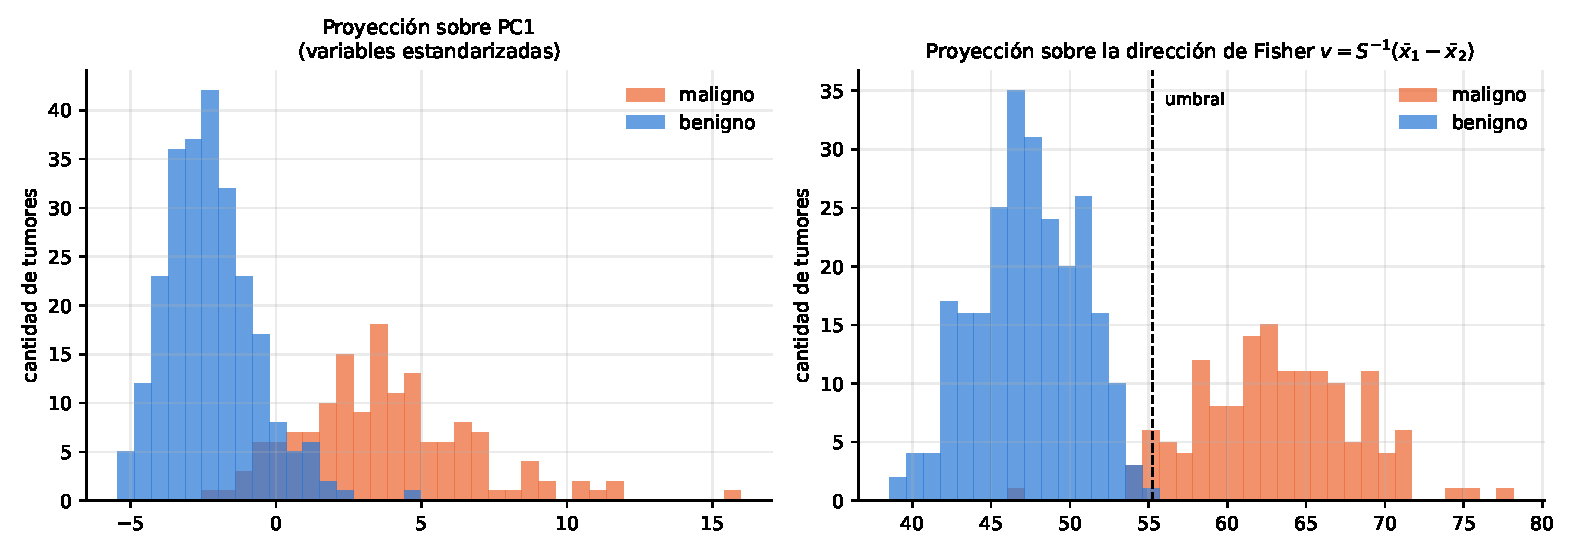
\includegraphics[width=\textwidth]{figuras/lda_mama_histogramas.pdf}
\caption{Tumores de mama, datos de entrenamiento: histogramas por clase de la
proyección sobre la primera componente principal (izquierda, con las
variables estandarizadas) y sobre la dirección de Fisher (derecha), con el
punto medio $c$ entre las dos medias proyectadas, que es la frontera de LDA.}
\label{lda-fig:mama}
\end{figure}

\begin{example}[Tumores de mama]\label{lda-ejem:mama}
Con los $398$ tumores de entrenamiento ($p=30$) se calculan la dirección de
Fisher, $\bi{w}=S^{-1}(\bar{\bi{x}}_{\text{mal}}-\bar{\bi{x}}_{\text{ben}})$, y el punto medio
$c$. En los $171$ tumores de prueba, la matriz de confusión es (filas: clase
verdadera; columnas: clase asignada; primero maligno y después benigno)
\[
K=\begin{pmatrix}58&6\\2&105\end{pmatrix}:
\]
LDA acierta $163$ de $171$, el $95{,}3\%$, contra el $91{,}2\%$ de la media
más cercana con las variables estandarizadas y el $90{,}1\%$ de PCA con una
componente. Además, de los $64$ tumores malignos, solo $6$ fueron
clasificados como benignos (con la media más cercana eran $8$). Como LDA no
depende de las unidades (Ejercicio~\ref{lda-ej:unidades}), el resultado es
exactamente el mismo con las variables estandarizadas o sin estandarizar. La Figura~\ref{lda-fig:mama}
muestra por qué anda mejor: proyectados sobre la dirección de Fisher, los
tumores de las dos clases se solapan mucho menos que sobre la primera
componente principal.
\end{example}


% =====================================================================
\section{Más de dos clases}\label{lda-sec:multi}

Con $C$ clases buscamos varias direcciones: dos para dibujar las clases en el
plano y, para clasificar, las que hagan falta. El criterio es el de dos
clases, sumado sobre todos los pares de clases. Proyectando sobre $\bi{w}$,
queremos:
\begin{itemize}[leftmargin=*,itemsep=1pt]
\item que las \textbf{medias proyectadas} queden lejos unas de otras. Para
cada par de clases $j<k$, como con dos clases,
\[
\bigl(\bi{w}\transp\bar{\bi{x}}_j-\bi{w}\transp\bar{\bi{x}}_k\bigr)^2=\bi{w}\transp(\bar{\bi{x}}_j-\bar{\bi{x}}_k)(\bar{\bi{x}}_j-\bar{\bi{x}}_k)\transp \bi{w} ,
\]
y el par cuenta $n_jn_k$ veces: tantas como pares de observaciones con una en
cada clase;
\item que cada \textbf{clase proyectada} sea compacta: $\bi{w}\transp S\bi{w}$ chico, como
antes.
\end{itemize}
Sumando sobre los pares y dividiendo por $n$, la primera cantidad resulta ser
la dispersión de las medias proyectadas alrededor de la media proyectada de
todos los datos, $\bi{w}\transp\bar{\bi{x}}$, con cada clase contada $n_k$ veces
(Ejercicio~\ref{lda-ej:SB}):
\[
\frac1n\sum_{j<k}n_jn_k\bigl(\bi{w}\transp\bar{\bi{x}}_j-\bi{w}\transp\bar{\bi{x}}_k\bigr)^2
=\sum_{k=1}^Cn_k\bigl(\bi{w}\transp\bar{\bi{x}}_k-\bi{w}\transp\bar{\bi{x}}\bigr)^2=\bi{w}\transp S_B\bi{w} ,
\]
otra vez una forma cuadrática, con la matriz que sigue.

\begin{definition}[Dispersión entre clases]\label{lda-def:SB}
La \textbf{matriz de dispersión entre clases} es
\[
S_B=\sum_{k=1}^Cn_k(\bar{\bi{x}}_k-\bar{\bi{x}})(\bar{\bi{x}}_k-\bar{\bi{x}})\transp\ \in\R^{p\times p}
\]
(la $B$ viene de \emph{between}, ``entre''). Es simétrica y semidefinida
positiva, y con dos clases es $S_B=\frac{n_1n_2}{n}\,\bi{a}\bi{a}\transp$, porque hay un
solo par.
\end{definition}

Fisher propone maximizar, como con dos clases,
\[
\frac{\bi{w}\transp S_B\bi{w}}{\bi{w}\transp S\bi{w}}.
\]
Es otra vez un cociente de Rayleigh generalizado, ahora con $A=S_B$ y $B=S$,
así que \emph{no hay nada nuevo que demostrar}. Sean
$\lambda_1\ge\dots\ge\lambda_p$ y $\bi{w}_1,\dots,\bi{w}_p$ los autovalores y los
autovectores generalizados de $(S_B,S)$, normalizados con
$\bi{w}_j\transp S\bi{w}_k=\delta_{jk}$. Por el Teorema~\ref{lda-teo:rayleigh}, la mejor
dirección es $\bi{w}_1$, con cociente $\lambda_1$; entre las direcciones
$S$-ortogonales a $\bi{w}_1$, la mejor es $\bi{w}_2$, con cociente $\lambda_2$; y así
siguiendo. Con dos clases, el cociente es $\frac{n_1n_2}{n}J(\bi{w})$, y $\bi{w}_1$ es
la dirección de Fisher. Lo único nuevo es cuántas de estas direcciones sirven.

\begin{proposition}[A lo sumo $C-1$ direcciones]\label{lda-prop:multi}
Los autovalores generalizados $\lambda_k$ de $(S_B,S)$ son mayores o iguales
que cero, y a lo sumo $C-1$ son positivos. Si $\lambda_k=0$, todas las medias
proyectadas sobre $\bi{w}_k$ coinciden: esa dirección no separa nada.
\end{proposition}

\begin{proof}
Sea $\bi{w}$ un autovector generalizado, $S_B\bi{w}=\lambda S\bi{w}$, con $\bi{w}\transp S\bi{w}=1$.
Multiplicando a izquierda por $\bi{w}\transp$,
\[
\lambda=\bi{w}\transp S_B\bi{w}=\sum_{k=1}^Cn_k\bigl(\bi{w}\transp\bar{\bi{x}}_k-\bi{w}\transp\bar{\bi{x}}\bigr)^2\ \ge0 ,
\]
y es cero solo si todas las medias proyectadas sobre $\bi{w}$ coinciden (con
$\bi{w}\transp\bar{\bi{x}}$). Como en la demostración del Teorema~\ref{lda-teo:rayleigh},
los $\lambda_k$ son los autovalores de la matriz simétrica
$H=S^{-1/2}S_BS^{-1/2}$, así que la cantidad de $\lambda_k$ no nulos es
$\rango(H)=\rango(S_B)$ (multiplicar por matrices invertibles no cambia el
rango). Con $d_k=\bar{\bi{x}}_k-\bar{\bi{x}}$, para todo $\bi{v}$ vale
$S_B\bi{v}=\sum_kn_kd_k\,(d_k\transp \bi{v})$, así que las columnas de $S_B$ están en
$\gen(d_1,\dots,d_C)$; y esos $C$ vectores son linealmente dependientes,
porque $\sum_kn_kd_k=\sum_kn_k\bar{\bi{x}}_k-n\bar{\bi{x}}=0$. Entonces
$\rango(S_B)\le\dim\gen(d_1,\dots,d_C)\le C-1$.
\end{proof}

Así, con $C$ clases hay a lo sumo $C-1$ \textbf{direcciones discriminantes}
útiles: una con dos clases, dos con tres (un plano), nueve con los diez
dígitos. Es razonable: las $C$ medias están en un subespacio afín de
dimensión $C-1$ como mucho, y fuera de él no hay nada que separar.

\begin{definition}[Regla de LDA]\label{lda-def:regla}
Sea $r$ la cantidad de autovalores generalizados positivos de $(S_B,S)$ (a lo
sumo $C-1$) y sea $W=[\,\bi{w}_1\ \cdots\ \bi{w}_r\,]\in\R^{p\times r}$. Cada observación
$\bi{x}$ se reemplaza por sus \textbf{coordenadas discriminantes}
$z=W\transp \bi{x}\in\R^r$, y se le asigna la clase $k$ cuya media está más cerca
en $\R^r$: la que hace mínima la distancia $\|W\transp \bi{x}-W\transp\bar{\bi{x}}_k\|$.
\end{definition}

Con dos clases, $r=1$ y es la regla de la Sección~\ref{lda-sec:clasificar};
para dibujar se usan las dos primeras coordenadas (LD1 y LD2). La
normalización importa: por el Teorema~\ref{lda-teo:rayleigh}(a),
$W\transp SW=I_r$ y $W\transp S_BW=\diag(\lambda_1,\dots,\lambda_r)$, así que en
las coordenadas $z$ la dispersión dentro de las clases es la misma en todas
las direcciones, y por eso se mide con la distancia euclídea. Que las dos
matrices queden diagonales a la vez es la diagonalización simultánea de la
Sección~\ref{lda-sec:simultanea}.

\begin{figure}[!htb]
\centering
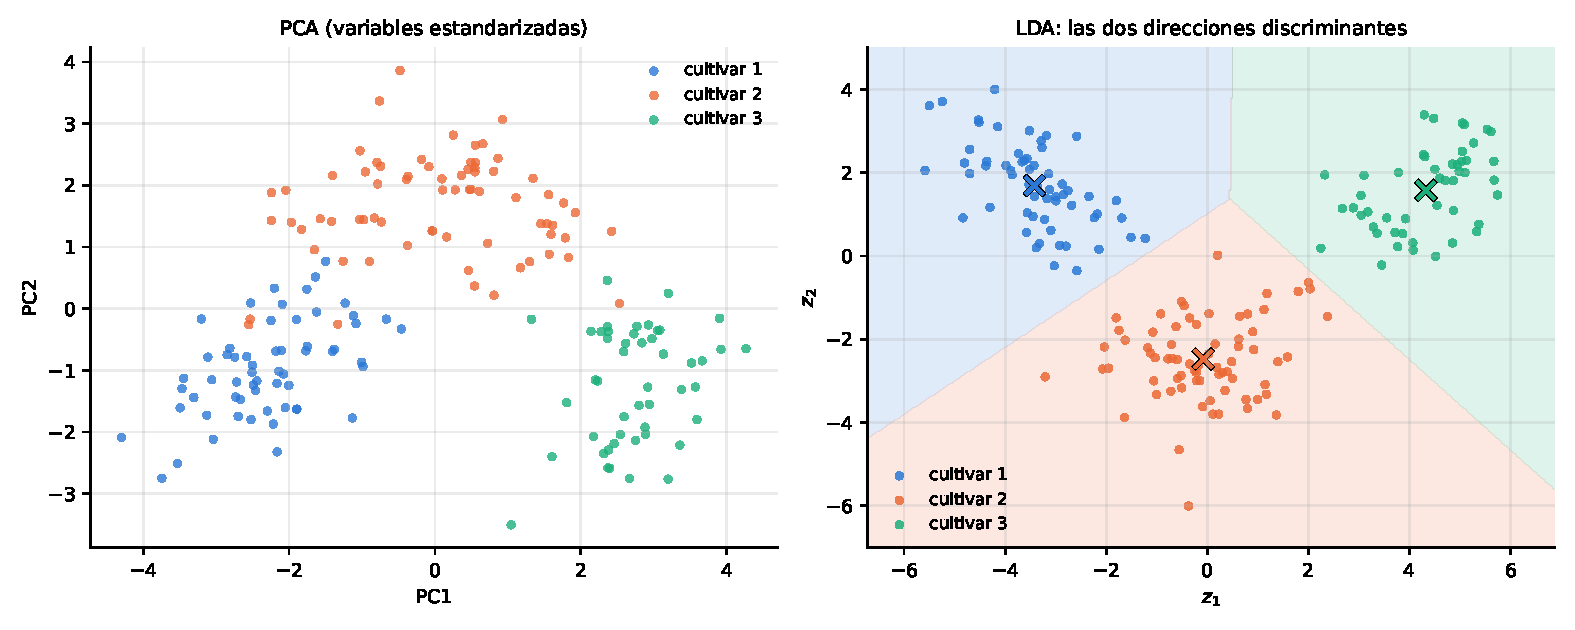
\includegraphics[width=\textwidth]{figuras/lda_vino_pca_lda.pdf}
\caption{Vinos ($n=178$, $p=13$, $C=3$ variedades; las dos figuras usan los
$178$ vinos). Izquierda: las dos primeras componentes principales de las
variables estandarizadas. Derecha: las dos coordenadas discriminantes de LDA
(normalizadas con la covarianza pooled), con las medias de las clases
($\times$) y las regiones de la regla de LDA, la media más cercana en ese
plano.}
\label{lda-fig:vino}
\end{figure}

\begin{example}[Vinos]\label{lda-ejem:vino}
En los vinos del capítulo anterior ($178$ vinos, $p=13$, $C=3$) hay a lo sumo
dos direcciones discriminantes; con todos los vinos, los autovalores
generalizados positivos de $(S_B,S)$ son $\lambda_1\approx9{,}08$ y
$\lambda_2\approx4{,}13$. La Figura~\ref{lda-fig:vino} compara el plano de PCA
con el de LDA: en el primero las clases se tocan, y en el segundo quedan bien
separadas. Para clasificar, todo se calcula con los $124$ vinos de
entrenamiento: la regla de LDA acierta los $54$ vinos de prueba ($100\%$),
contra el $98{,}1\%$ de la media más cercana con las variables estandarizadas
y el $68{,}5\%$ sin estandarizar (con una sola coordenada discriminante, LDA
acierta el $94{,}4\%$). Con o sin estandarizar, LDA asigna las mismas clases
(Ejercicio~\ref{lda-ej:unidades}).
\end{example}

\begin{example}[Dígitos]\label{lda-ejem:digitos}
Con los diez dígitos hay hasta nueve direcciones discriminantes (antes hay que
sacar los cuatro píxeles que valen $0$ en todas las imágenes de entrenamiento,
porque con ellos $S$ no es invertible: Observación~\ref{lda-rem:invertible}).
Con las nueve, LDA acierta el $95{,}9\%$ de los dígitos de prueba, contra el
$88{,}3\%$ de la media más cercana con nueve componentes principales y el
$90{,}4\%$ con los $64$ píxeles: nueve números por imagen, bien elegidos,
alcanzan.
\end{example}

La Tabla~\ref{lda-tab:pca-lda} pone lado a lado PCA, del capítulo anterior, y LDA.

\begin{table}[!ht]
\centering
\small\renewcommand{\arraystretch}{1.3}
\begin{tabular}{@{}p{3.1cm}p{5.4cm}p{5.4cm}@{}}
\toprule
 & PCA & LDA\tabularnewline
\midrule
\raggedright usa las etiquetas & \raggedright no & \raggedright sí\tabularnewline
\raggedright qué busca & \raggedright máxima varianza: $\|X_c\bi{w}\|^2$, con $\|\bi{w}\|=1$ & \raggedright máxima separación relativa: $\dfrac{\bi{w}\transp S_B\bi{w}}{\bi{w}\transp S\bi{w}}$\tabularnewline
\raggedright cómo se calcula & \raggedright SVD de la matriz centrada $X_c$ & \raggedright autovectores generalizados de $(S_B,S)$\tabularnewline
\raggedright las direcciones son & \raggedright ortonormales & \raggedright $S$-ortonormales\tabularnewline
\raggedright cuántas & \raggedright hasta el rango de $X_c$ & \raggedright hasta $C-1$\tabularnewline
\raggedright cambiar las unidades & \raggedright cambia el resultado & \raggedright no cambia nada\tabularnewline
\raggedright sirve para & \raggedright describir, comprimir, dibujar & \raggedright separar y clasificar\tabularnewline
\bottomrule
\end{tabular}
\caption{PCA y LDA, lado a lado.}
\label{lda-tab:pca-lda}
\end{table}

% =====================================================================
\section{Otra aplicación: la diagonalización simultánea}\label{lda-sec:simultanea}

La parte (a) del Teorema~\ref{lda-teo:rayleigh}, escrita con matrices, dice algo que
vale la pena mirar por sí mismo: \emph{dos} formas cuadráticas, una de ellas
definida positiva, se pueden diagonalizar a la vez con un mismo cambio de base.

\begin{theorem}[Diagonalización simultánea por congruencia]\label{lda-teo:simultanea}
Si $A$ es simétrica y $B$ es simétrica definida positiva, hay una matriz
invertible $W$ tal que
\[
W\transp BW=I,\qquad W\transp AW=\Lambda=\diag(\lambda_1,\dots,\lambda_p),
\]
donde $\lambda_1,\dots,\lambda_p$ son los autovalores generalizados de $(A,B)$.
Las columnas de $W$ son los autovectores generalizados $\bi{w}_1,\dots,\bi{w}_p$ del
Teorema~\ref{lda-teo:rayleigh}(a).
\end{theorem}

\begin{proof}
Como en la demostración del Teorema~\ref{lda-teo:rayleigh}, sea
$H=B^{-1/2}AB^{-1/2}$, que es simétrica. Por el teorema espectral,
$H=Q\Lambda Q\transp$, con $Q=[\,y_1\ \cdots\ y_p\,]$ ortogonal y
$\Lambda=\diag(\lambda_1,\dots,\lambda_p)$. Sea $W=B^{-1/2}Q$, que es invertible
porque es un producto de matrices invertibles. Entonces
\begin{align*}
W\transp BW&=Q\transp B^{-1/2}BB^{-1/2}Q=Q\transp Q=I,\\
W\transp AW&=Q\transp B^{-1/2}AB^{-1/2}Q=Q\transp HQ=\Lambda ,
\end{align*}
y las columnas de $W$ son los $\bi{w}_k=B^{-1/2}y_k$ del Teorema~\ref{lda-teo:rayleigh}(a).
\end{proof}

Con el cambio de variables $\bi{w}=W\xi$, las dos formas cuadráticas quedan
diagonales \emph{en la misma base}:
\[
\bi{w}\transp B\bi{w}=\xi_1^2+\dots+\xi_p^2,\qquad \bi{w}\transp A\bi{w}=\lambda_1\xi_1^2+\dots+\lambda_p\xi_p^2 .
\]
En LDA ya lo usamos: en las coordenadas discriminantes, $S$ pasa a ser la
identidad y $S_B$ pasa a ser diagonal (Sección~\ref{lda-sec:multi}).

\paragraph{Congruencia, no semejanza.} En el teorema aparece $W\transp(\cdot)W$,
no $W^{-1}(\cdot)W$: es una \emph{congruencia}, que conserva la simetría pero
no los autovalores. En el Ejemplo~\ref{lda-ejem:strang}, los autovalores de $A$
son $2$ y $6$, y los de $\Lambda=W\transp AW$ son $3\pm\sqrt3$: otros números,
pero los mismos signos. Eso pasa siempre: una congruencia conserva cuántos
autovalores son positivos, cuántos negativos y cuántos nulos (es la ley de
inercia de Sylvester, que no demostramos).

\paragraph{¿Dónde se usa?} Un ejemplo de \emph{machine learning}: las
interfaces cerebro--computadora. Se registra la actividad eléctrica del cerebro
(un electroencefalograma) con $p$ electrodos mientras una persona imagina que
mueve la mano izquierda (clase~1) o la derecha (clase~2), y se calculan las
matrices de covarianza $\Sigma_1$ y $\Sigma_2$ de las $p$ señales en cada clase.
El método CSP (\emph{common spatial patterns}) busca combinaciones de los
electrodos, $\bi{w}\transp \bi{x}$, cuya varianza sea grande en una clase y chica en la
otra: el máximo y el mínimo de $\bi{w}\transp\Sigma_1\bi{w}/\bi{w}\transp\Sigma_2\bi{w}$, que es un
cociente de Rayleigh generalizado. Por el Teorema~\ref{lda-teo:rayleigh}, esas
combinaciones son las columnas de la matriz $W$ que diagonaliza a la vez las
dos covarianzas, $W\transp\Sigma_2W=I$ y $W\transp\Sigma_1W=\Lambda$, y se usan
las de $\lambda_k$ más grande y más chico. Las varianzas de esas pocas
combinaciones son después las variables para decidir, por ejemplo con LDA, si
la persona pensó en la mano izquierda o en la derecha \cite{BTLKM2008}.

% =====================================================================
\section*{Videos}
\begin{itemize}
\item \href{https://youtu.be/HgtUtNUQ4tk}{\textbf{Video 26: Cociente de Rayleigh y autovalores generalizados}} (18 min).
Definición de cociente de Rayleigh. Equivalencia en la maximización y
minimización con el cociente de Rayleigh con denominador igual a la
identidad. ¿Cómo se traduce la ortogonalidad del caso clásico en este caso?
(Sección~\ref{lda-sec:rayleigh}.)
% COMPLETAR: si hay videos de LDA y clasificación, agregarlos acá.
\end{itemize}

% =====================================================================
\begin{ideas}[frametitle={Ideas clave},frametitlefont=\bfseries\large,frametitlebelowskip=4pt]
\begin{itemize}[leftmargin=*,itemsep=2pt]
\item \textbf{Fisher, con matrices}: las medias proyectadas lejos,
$(\bi{w}\transp \bi{a})^2=\bi{w}\transp(\bi{a}\bi{a}\transp)\bi{w}$, y cada clase proyectada compacta,
$\|\tilde X\bi{w}\|^2=\bi{w}\transp S\bi{w}$; el cociente de Fisher es
$J(\bi{w})=\bi{w}\transp(\bi{a}\bi{a}\transp)\bi{w}/\bi{w}\transp S\bi{w}$.
\item \textbf{Rayleigh generalizado}: el máximo de $\bi{w}\transp A\bi{w}/\bi{w}\transp B\bi{w}$ es
el mayor autovalor de $A\bi{w}=\lambda B\bi{w}$. Con $y=B^{1/2}\bi{w}$ el denominador pasa a
ser $y\transp y$, y es el problema de la matriz simétrica
$H=B^{-1/2}AB^{-1/2}$. Hay una base de autovectores generalizados
$B$-ortogonales.
\item \textbf{La dirección de Fisher es un caso particular}: con $A=\bi{a}\bi{a}\transp$,
de rango uno, el único autovalor no nulo es $\bi{a}\transp S^{-1}\bi{a}$, con
autovector $\bi{w}^\ast=S^{-1}(\bar{\bi{x}}_1-\bar{\bi{x}}_2)$.
\item \textbf{Clasificar}: se proyecta sobre $\bi{w}^\ast$ y se corta en el punto
medio de las medias proyectadas; la frontera es un hiperplano perpendicular a
$\bi{w}^\ast$.
\item \textbf{$C$ clases}: como con dos, sumando sobre los pares de clases (cada
par cuenta $n_jn_k$ veces), las medias proyectadas separadas,
$\frac1n\sum_{j<k}n_jn_k(\bi{w}\transp\bar{\bi{x}}_j-\bi{w}\transp\bar{\bi{x}}_k)^2=\bi{w}\transp S_B\bi{w}$, con
$S_B=\sum_kn_k(\bar{\bi{x}}_k-\bar{\bi{x}})(\bar{\bi{x}}_k-\bar{\bi{x}})\transp$; y cada clase compacta,
$\bi{w}\transp S\bi{w}$. Es el mismo teorema con $A=S_B$: las
direcciones son los autovectores generalizados de $(S_B,S)$, y sirven a lo
sumo $C-1$, porque $\rango(S_B)\le C-1$.
\item \textbf{Diagonalización simultánea}: con $H=B^{-1/2}AB^{-1/2}=Q\Lambda Q\transp$
y $W=B^{-1/2}Q$, $W\transp BW=I$ y $W\transp AW=\Lambda$ (congruencia, no
semejanza). Se usa, por ejemplo, en las interfaces
cerebro--computadora (CSP).
\end{itemize}
\end{ideas}

% =====================================================================
\section*{Ejercicios}
\addcontentsline{toc}{section}{Ejercicios}

\noindent\footnotesize \textsc{[Cálculo]} para fijar la mecánica,
\textsc{[Concepto]} para justificar y demostrar (la computadora se usa en la
práctica). Los ejercicios~\ref{lda-ej:strang1}, \ref{lda-ej:strang2},
\ref{lda-ej:strang4}, \ref{lda-ej:strang8} y~\ref{lda-ej:congruencias} son de
la Sección I.10 de Strang (con algunos
agregados), escritos con la notación del capítulo: $A$ en el numerador y $B$ en
el denominador (Strang usa $S$ y $M$).\normalsize

\begin{enumerate}[leftmargin=*,label=\textbf{\thechapter.\arabic*},ref=\thechapter.\arabic*,itemsep=4pt]

% ---------- El cociente de Rayleigh generalizado (Strang I.10) ----------
\item \tipo{Cálculo}\label{lda-ej:strang1} Resolver $(A-\lambda B)\bi{x}=0$ y
$(H-\lambda I)y=0$, después de calcular $H=B^{-1/2}AB^{-1/2}$, para
\[
A=\begin{pmatrix}5&4\\4&5\end{pmatrix},\qquad B=\begin{pmatrix}1&0\\0&4\end{pmatrix}.
\]
Primero hallar $\lambda_1$ y $\lambda_2$ de $\det(A-\lambda B)=0$; la ecuación
$\det(H-\lambda I)=0$ debería dar los mismos valores. Verificar que
$\bi{x}_1\transp \bi{x}_2\ne0$ pero $\bi{x}_1\transp B\bi{x}_2=0$, y que $y_1\transp y_2=0$ porque
$H$ es simétrica. ¿Cómo se relacionan los autovectores $\bi{x}_1,\bi{x}_2$ con los
autovectores $y_1,y_2$?

\item \tipo{Cálculo}\label{lda-ej:strang2}
\begin{enumerate}[label=(\alph*)]
\item Para $\bi{x}=(\bi{a},\bi{b})$ e $y=(c,d)$, escribir los cocientes del ejercicio
anterior como
\[
R^\ast(\bi{x})=\frac{\bi{x}\transp A\bi{x}}{\bi{x}\transp B\bi{x}}=\frac{5\bi{a}^2+8\bi{a}\bi{b}+5\bi{b}^2}{\bi{a}^2+4\bi{b}^2},\qquad
R(y)=\frac{y\transp Hy}{y\transp y}=\frac{5c^2+4cd+\frac54d^2}{c^2+d^2}.
\]
% NOTA (revisión): en el libro de Strang el numerador de R(y) aparece como
% 5c^2+16cd+20d^2, que corresponde a M^{1/2} S M^{1/2} y no a H = M^{-1/2} S M^{-1/2}
% (en la notación de Strang: S es nuestra A y M es nuestra B).
% Con H = [[5,2],[2,5/4]] el numerador correcto es 5c^2+4cd+(5/4)d^2.
\item Derivar $R(y)$ respecto de $c$ y de $d$ para encontrar su máximo y su
mínimo.
\item Lo mismo con $R^\ast(\bi{x})$ respecto de $\bi{a}$ y de $\bi{b}$.
\item Verificar que los máximos se alcanzan en autovectores de
$(A-\lambda B)\bi{x}=0$ y de $(H-\lambda I)y=0$.
\end{enumerate}

\item \tipo{Cálculo}\label{lda-ej:strang4} En el
Ejercicio~\ref{lda-ej:strang1}, cambiar $B$ por
$\left(\begin{smallmatrix}1&0\\0&0\end{smallmatrix}\right)$ y resolver
$A\bi{x}=\lambda B\bi{x}$. Ahora $B$ es singular: hay un $\bi{x}_2\ne0$ con $B\bi{x}_2=0$, sobre el
que el cociente $\bi{x}\transp A\bi{x}/\bi{x}\transp B\bi{x}$ no está definido (``vale
infinito''), y se dice que uno de los autovalores es infinito. Verificar que
$\bi{x}_2$ sigue siendo $B$-ortogonal al autovector $\bi{x}_1$ del otro autovalor.

\item \tipo{Concepto} \textbf{$B$-ortogonales, directamente.}\label{lda-ej:Bortogonal}
Sin usar $B^{1/2}$, probar que si $A\bi{w}_1=\lambda_1B\bi{w}_1$, $A\bi{w}_2=\lambda_2B\bi{w}_2$ y
$\lambda_1\ne\lambda_2$, entonces $\bi{w}_1\transp B\bi{w}_2=0$ y también
$\bi{w}_1\transp A\bi{w}_2=0$. (Sugerencia: multiplicar la primera ecuación a izquierda
por $\bi{w}_2\transp$ y la segunda por $\bi{w}_1\transp$, y usar que $A$ y $B$ son
simétricas, como para los autovectores de una matriz simétrica, que es el caso
$B=I$.)

% ---------- La dirección de Fisher ----------
\item \tipo{Concepto} \textbf{La dirección de Fisher, de dos maneras.}\label{lda-ej:strang8}
(Strang.) Sean $\bi{u}\in\R^p$ no nulo, $B$ definida positiva y
$R(\bi{x})=\bi{x}\transp A\bi{x}/\bi{x}\transp B\bi{x}$ con $A=\bi{u}\bi{u}\transp$, que es el problema de Fisher.
\begin{enumerate}[label=(\alph*)]
\item ¿Qué vector $\bi{x}$ maximiza $R(\bi{x})$? ¿Cuánto vale el máximo? (Usar el
Corolario~\ref{lda-cor:fisher} con $\bi{u}$ en lugar de $\bi{a}$ y $B$ en lugar de
$S$: su demostración solo usa que $S$ es definida positiva.) Si $p\ge2$,
¿cuánto vale el mínimo, y dónde se alcanza?
\item Otra demostración del máximo, sin autovalores, que es la de la
desigualdad de Cauchy--Schwarz del Capítulo~\ref{cap:ortogonalidad}: con
$\bi{v}=B^{-1}\bi{u}$, desarrollar $0\le(\bi{x}-t\bi{v})\transp B(\bi{x}-t\bi{v})$ como un polinomio de
grado dos en $t$, y usar que su discriminante es menor o igual que cero para
probar que $(\bi{u}\transp \bi{x})^2\le(\bi{u}\transp B^{-1}\bi{u})\,(\bi{x}\transp B\bi{x})$.
\item Probar que vale la igualdad si y solo si $\bi{x}$ es un múltiplo de
$B^{-1}\bi{u}$. Deducir que el máximo del cociente de Fisher se alcanza solo en
los múltiplos de $\bi{w}^\ast$.
\end{enumerate}

\item \tipo{Cálculo} \textbf{Los ocho puntos.}\label{lda-ej:ocho} Con los datos
de los Ejemplos~\ref{lda-ejem:ocho} a~\ref{lda-ejem:ocho-regla}:
\begin{enumerate}[label=(\alph*)]
\item Verificar $S=\tilde X\transp \tilde X$, $S^{-1}$, la dirección de Fisher y
$J_{\max}=4{,}5$. Calcular $J(\bi{e}_2)$ y $J\bigl((3,-1)\bigr)$.
\item Calcular $S_B$ y resolver $\det(S_B-\lambda S)=0$: ¿cuáles son los dos
autovalores generalizados? ¿Cómo se relaciona el mayor con $J_{\max}$?
\item Clasificar los puntos $(2,0)$, $(1,-2)$ y $(0,-1)$ con LDA y con la media
más cercana del capítulo anterior. ¿En cuáles difieren? ¿Qué pasa con $(3,3)$?
\end{enumerate}

\item \tipo{Concepto} \textbf{La matriz $S$.}\label{lda-ej:SW}
\begin{enumerate}[label=(\alph*)]
\item Probar que $\tilde X\transp \tilde X=\sum_k\sum_{i:\,y_i=k}(\bi{x}_i-\bar{\bi{x}}_k)(\bi{x}_i-\bar{\bi{x}}_k)\transp$.
\item Probar que $S\bi{w}=0$ si y solo si $\tilde X\bi{w}=0$, y que esto pasa si y solo si
cada clase, proyectada sobre $\gen(\bi{w})$, queda en un solo punto.
\item Si $G$ es la matriz indicadora de las clases del capítulo anterior,
probar que $G\transp \tilde X=0$. Deducir que $\rango(\tilde X)\le n-C$ y que, si
$p>n-C$, $S$ no es invertible.
\end{enumerate}

\item \tipo{Concepto} \textbf{La dispersión entre clases, de otra
manera.}\label{lda-ej:SB} Sea $\bar{\bi{x}}=\frac1n\sum_kn_k\bar{\bi{x}}_k$ la media de
todos los datos.
\begin{enumerate}[label=(\alph*)]
\item Probar que
\[
S_B=\frac1n\sum_{j<k}n_jn_k\,(\bar{\bi{x}}_j-\bar{\bi{x}}_k)(\bar{\bi{x}}_j-\bar{\bi{x}}_k)\transp ,
\]
y deducir la igualdad de la Sección~\ref{lda-sec:multi},
\[
\frac1n\sum_{j<k}n_jn_k\bigl(\bi{w}\transp\bar{\bi{x}}_j-\bi{w}\transp\bar{\bi{x}}_k\bigr)^2=\sum_kn_k\bigl(\bi{w}\transp\bar{\bi{x}}_k-\bi{w}\transp\bar{\bi{x}}\bigr)^2 .
\]
(Sugerencia: desarrollar los productos en la suma sobre \emph{todos} los
pares $(j,k)$, que es el doble de la suma sobre $j<k$, y usar que
$\sum_kn_k\bar{\bi{x}}_k=n\bar{\bi{x}}$.)
\item Probar que $S_B=\bar X\transp\bar X$, donde $\bar X\in\R^{n\times p}$ es la
matriz cuya fila $i$ es $(\bar{\bi{x}}_{y_i}-\bar{\bi{x}})\transp$: cada observación
reemplazada por la media de su clase, menos la media de todos los datos.
\item Con dos clases, probar que $\bi{w}^\ast=S^{-1}\bi{a}$ es autovector generalizado
de $(S_B,S)$ con autovalor $\frac{n_1n_2}{n}\,\bi{a}\transp S^{-1}\bi{a}$. ¿Cuánto valen
los demás autovalores generalizados?
\end{enumerate}

\item \tipo{Concepto} \textbf{Las unidades.}\label{lda-ej:unidades}
Cada observación $\bi{x}$ se reemplaza por $\bi{x}'=T\bi{x}+\bi{b}$, con $T$ invertible.
\begin{enumerate}[label=(\alph*)]
\item Probar que las medias nuevas son $T\bar{\bi{x}}_k+\bi{b}$ y que
$\tilde X'=\tilde XT\transp$, y deducir que $S'=TST\transp$ y
$S_B'=TS_BT\transp$.
\item Con dos clases, probar que la dirección de Fisher nueva es
$T^{-\top}\bi{w}^\ast$, donde $T^{-\top}=(T^{-1})\transp$, que
\[
(T^{-\top}\bi{w}^\ast)\transp \bi{x}'=\bi{w}^{\ast\top}\bi{x}+\bi{w}^{\ast\top}T^{-1}\bi{b}\qquad\text{para todo }\bi{x},
\]
y que la regla de LDA asigna las mismas clases.
\item Con $C$ clases, probar que si $S_B\bi{w}=\lambda S\bi{w}$, entonces
$S_B'(T^{-\top}\bi{w})=\lambda\,S'(T^{-\top}\bi{w})$: los autovalores generalizados no
cambian, y las direcciones pasan a ser los $T^{-\top}\bi{w}_k$, con la misma
normalización. Deducir que las coordenadas discriminantes solo se corren en
una constante, y que la regla de LDA asigna las mismas clases.
\item En cambio, en PCA las unidades importan: con los puntos $(1,1)$,
$(-1,-1)$, $(\frac12,-\frac12)$ y $(-\frac12,\frac12)$, calcular la primera
dirección principal antes y después de multiplicar la primera variable por
$10$.
\end{enumerate}

\item \tipo{Cálculo} \textbf{Tres clases redondas.}\label{lda-ej:tres} Con las
tres clases del ejercicio ``Tres clases a mano'' del capítulo anterior (la
clase A son los puntos $(0,0)$, $(2,0)$, $(0,2)$, $(2,2)$; la clase B,
$(5,0)$, $(7,0)$, $(5,2)$, $(7,2)$; y la clase C, $(2,5)$, $(4,5)$, $(2,7)$,
$(4,7)$):
\begin{enumerate}[label=(\alph*)]
\item Verificar que $S=12I$: las clases son ``redondas''. Deducir que las
direcciones discriminantes son autovectores de $S_B$, y calcularlas, junto con
los autovalores generalizados (a mano o con la computadora: los números no son
redondos).
\item Como $p=2=C-1$, la matriz $W$ es de $2\times2$. Probar que
$W=\frac1{\sqrt{12}}Q$, con $Q$ ortogonal, y deducir que la regla de LDA
asigna las mismas clases que la media más cercana en el plano. ¿Por qué era de
esperar, si las clases son redondas?
\end{enumerate}

\item \tipo{Concepto} \textbf{Regularizar.}\label{lda-ej:regularizar} Sea
$\bi{w}_\varepsilon=(S+\varepsilon I)^{-1}\bi{a}$, con $\bi{a}=\bar{\bi{x}}_1-\bar{\bi{x}}_2$ y
$\varepsilon>0$.
\begin{enumerate}[label=(\alph*)]
\item Probar que $S+\varepsilon I$ es definida positiva aunque $S$ no sea
invertible.
\item Si $S=Q\Lambda Q\transp$, escribir $\bi{w}_\varepsilon$ en la base de los
autovectores de $S$.
\item Probar que $\varepsilon \bi{w}_\varepsilon\to \bi{a}$ cuando
$\varepsilon\to\infty$ (la regla se parece cada vez más a la de la media más
cercana) y que $\bi{w}_\varepsilon\to S^{-1}\bi{a}$ cuando $\varepsilon\to0$, si $S$
es invertible.
\end{enumerate}

% ---------- La diagonalización simultánea ----------
\item \tipo{Concepto} \textbf{Diagonalización simultánea: la
recíproca.}\label{lda-ej:simultanea} Probar que si $Z$ es invertible,
$Z\transp BZ=I$ y $Z\transp AZ=\Lambda$ es diagonal, entonces $AZ=BZ\Lambda$: las
columnas de $Z$ son autovectores generalizados de $(A,B)$, y los elementos de
la diagonal de $\Lambda$ son los autovalores generalizados. (Sugerencia: de
$Z\transp BZ=I$ sale que $(Z\transp)^{-1}=BZ$.)

\item \tipo{Concepto} \textbf{Congruencias.}\label{lda-ej:congruencias} (Strang.)
\begin{enumerate}[label=(\alph*)]
\item ¿Por qué toda congruencia $Z\transp AZ$ preserva la simetría de $A$?
\item ¿Por qué $Z\transp BZ$ es definida positiva si $B$ lo es y $Z$ es cuadrada
e invertible? Aplicar el test de energía a $Z\transp BZ$, sin olvidar explicar
por qué $Z\bi{x}$ no es el vector cero.
\item ¿Qué matrices son congruentes a la identidad, es decir, de la forma
$Z\transp IZ$ con $Z$ invertible?
\end{enumerate}

\end{enumerate}

% =====================================================================
\section*{Práctica: LDA versus PCA}
\addcontentsline{toc}{section}{Práctica: LDA versus PCA}
% =====================================================================

Los datos son los de la práctica del capítulo anterior (tumores de mama,
dígitos, cáncer de pulmón y siluetas de vehículos), con la misma separación en
entrenamiento y prueba (\texttt{separar(X, y)}, con la misma semilla) y los
mismos archivos \texttt{datos\_clasificacion.py} y
\texttt{herramientas\_clasificacion.py}. El objetivo es comparar PCA y LDA,
para dibujar las clases y para clasificar. El informe se entrega en una
notebook de Colab, con el código, los gráficos (con ejes y títulos) y las
respuestas, escritas en celdas de texto.

\paragraph{Antes de empezar.} Saque las columnas que son constantes en el
entrenamiento (con \texttt{columnas\_no\_constantes}; en el punto~\ref{lda-p:dos},
las que son constantes en las dos clases elegidas): si no, $S$ no es
invertible. Con el cáncer de pulmón, $S$ no es invertible ni así (hay más
variables que datos: Observación~\ref{lda-rem:invertible}): en los puntos L.2 a
L.5 use $S+\varepsilon I$ con $\varepsilon$ chico (por ejemplo,
$\varepsilon=10^{-3}\tr(S)/p$), que es definida positiva
(Ejercicio~\ref{lda-ej:regularizar}), y vea el punto L.6.

\begin{enumerate}[leftmargin=*,label=\textbf{L.\arabic*},ref=L.\arabic*,itemsep=6pt]

\item \textbf{Lo que ya tenemos.} Retome la investigación preliminar, los
gráficos exploratorios, el gráfico de PC1 contra PC2 y los aciertos de la
media más cercana (con y sin PCA) de la práctica anterior.

\item \textbf{LDA con dos clases.}\label{lda-p:dos} Con dos clases hay una sola
dirección. Use los tumores de mama (o, si su conjunto tiene más clases, elija
dos: por ejemplo, los dígitos $3$ y $8$, o los dos autos de los vehículos).
\begin{itemize}[itemsep=1pt]
\item Calcule $S$, la matriz de dispersión dentro de las clases (o la
covarianza pooled $S/(n-2)$, que da la misma dirección:
Observación~\ref{lda-rem:pooled}).
\item Calcule $\bi{w}=S^{-1}(\bar{\bi{x}}_1-\bar{\bi{x}}_2)$ resolviendo el sistema
$S\bi{w}=\bar{\bi{x}}_1-\bar{\bi{x}}_2$; no invierta $S$ (use \texttt{np.linalg.solve}).
\item Proyecte: $X\bi{w}\in\R^n$ es un número por individuo. Es el producto
matricial \texttt{X @ w}, no el producto entrada por entrada \texttt{X * w}
(que da una matriz de $n\times p$).
\item Haga histogramas de $X\bi{w}$ separados por clase, en entrenamiento y en
prueba, y compárelos con los de la proyección sobre PC1.
\item Clasifique con la media más cercana en la recta (cortando en el punto
medio $c$ de las medias proyectadas) y calcule los aciertos y la matriz de
confusión en prueba. Compare con la práctica anterior.
\end{itemize}

\item \textbf{LDA con más de dos clases.}\label{lda-p:multi} Si su conjunto
tiene más de dos clases:
\begin{itemize}[itemsep=1pt]
\item Calcule $S_B$ y las direcciones de LDA con la fórmula
$W=S^{-1/2}V$, donde $V$ tiene los autovectores de
$H=S^{-1/2}S_BS^{-1/2}$ con autovalor positivo
(como en la demostración del Teorema~\ref{lda-teo:rayleigh}, con $A=S_B$ y
$B=S$). ¿Cuántos
autovalores positivos hay? ¿Por qué?
\item Verifique numéricamente que $W\transp SW=I$ y que $W\transp S_BW$ es
diagonal. Compare con lo que da \texttt{scipy.linalg.eigh(S\_B, S)}: ¿son las
mismas direcciones?
\item Grafique los datos en las dos primeras coordenadas discriminantes (LD1
contra LD2), coloreados por clase, y compare con el gráfico de PC1 contra PC2.
\end{itemize}

\item \textbf{Clasificar.} Clasifique los datos de prueba con la regla de LDA
(la media más cercana en las coordenadas discriminantes): con todas las
coordenadas, y también con solo dos. Informe los aciertos y la matriz de
confusión, y compárelos con los de la práctica anterior (media más cercana en
$\R^p$, y PCA $+$ media más cercana con la misma cantidad de componentes).
Todo se calcula con el entrenamiento y se aplica, sin recalcular, a la prueba.

\item \textbf{Las unidades.} Multiplique una de las variables por $1000$ (un
cambio de unidades) y repita PCA y LDA. ¿Qué cambia y qué no?
(Ejercicio~\ref{lda-ej:unidades}.) Si usó $S+\varepsilon I$, ¿sigue
valiendo exactamente? ¿Por qué?

\item \textbf{Más variables que datos.} Con el cáncer de pulmón ($n=32$,
$p=56$): ¿qué rango tiene $S$? ¿Qué pasa al intentar resolver
$S\bi{w}=\bar{\bi{x}}_k-\bar{\bi{x}}_j$? Pruebe (i) reducir primero con PCA a $d$ componentes,
con $d$ menor o igual que la cantidad de datos de entrenamiento menos $C$, y
después hacer LDA, y (ii) regularizar, $S+\varepsilon I$. Compare los aciertos
en el entrenamiento y en la prueba, repitiendo todo con varias semillas, como
en la práctica anterior. ¿Qué concluye?

\item \textbf{Conclusiones.} ¿Qué método y qué dimensión elegiría para su
conjunto de datos, y por qué? ¿Qué gráfico muestra mejor las clases?

\item \textbf{(Opcional)} Compare con \texttt{scikit-learn}: la clase
\texttt{LinearDiscriminantAnalysis} del módulo
\texttt{sklearn.discriminant\_analysis}, con \texttt{priors} iguales para
todas las clases. ¿Asigna las mismas clases que la regla de LDA con todas las
coordenadas discriminantes?

\end{enumerate}

\subsection*{Los archivos de Python}

\begin{itemize}[leftmargin=*,itemsep=2pt]
\raggedright
\item \texttt{herramientas\_clasificacion.py} (el mismo de la práctica
anterior) tiene también las funciones de LDA: \texttt{dispersiones} ($S$,
$S_B$ y $X_c\transp X_c$), \texttt{covarianza\_pooled} ($S/(n-C)$), \texttt{direccion\_fisher} y
\texttt{umbral\_fisher} (el punto medio $c$; punto~\ref{lda-p:dos}),
\texttt{raiz\_inversa} y \texttt{lda\_practica} (la fórmula $S^{-1/2}V$ del
punto~\ref{lda-p:multi}), \texttt{lda\_autovalores} (lo mismo con
\texttt{scipy.linalg.eigh}) y \texttt{clasificar\_lda} (la media más cercana
en las coordenadas discriminantes); y, de la práctica anterior,
\texttt{columnas\_no\_constantes}.
\end{itemize}
% PARA EL DOCENTE (no se distribuye): practica11_lda.py es una resolución
% completa de la práctica; "python practica11_lda.py mama" guarda los gráficos
% en resultados_lda_mama/ y escribe los resultados.

% =====================================================================
